% !TeX program = lualatex

\documentclass[12pt]{article}



\usepackage[margin=1in]{geometry} 
\usepackage{amsmath,amsthm,amssymb}
\usepackage{MnSymbol}
\usepackage{graphicx}
\usepackage{bm}
\usepackage[normalem,normalbf]{ulem}
\usepackage{algorithm} 
\usepackage{algpseudocode} 
\usepackage{multirow}
\usepackage{rotating}
\usepackage{therefore}

\usepackage{tikz}
\usetikzlibrary{shapes.multipart}
\usetikzlibrary{shapes.symbols}

\usetikzlibrary{graphs,graphdrawing,graphs.standard,quotes}
\usegdlibrary{circular,force,layered,routing}
\tikzset{
	graphs/simpleer/.style={
		nodes={draw,circle, blue, left color=blue!20, text=black, inner sep=1pt},
		node distance=2.5cm, nodes={minimum size=2em}
	},
	every loop/.style={},
}

\newcommand*\circled[1]{\tikz[baseline=(char.base)]{
		\node[shape=circle,draw,inner sep=2pt] (char) {#1};}}

\newcommand{\m}{\medskip\\}
\newcommand{\N}{\mathbb{N}}
\newcommand{\Z}{\mathbb{Z}}
\newcommand{\R}{\mathbb{R}}
\newcommand{\bbs}{\textbackslash\textbackslash\space}
\newcommand{\bs}{\textbackslash\space}
\newcommand{\la}{\enskip\land\enskip}
\newcommand{\lo}{\enskip\lor\enskip}
\newcommand{\comp}[1]{#1^\mathsf{c}}
\newcommand{\micdrop}{\qed}
\newcommand{\contra}{\begin{tikzpicture}
		\node[starburst, draw, minimum width=3cm, minimum height=2cm,line width=1.5pt,red,fill=yellow,scale=.5]
		{BOOM, A CONTRADICTION!!!};
\end{tikzpicture}}

\renewcommand{\qedsymbol}{$\blacksquare$}

\DeclareMathOperator{\lcm}{lcm}

\newtheorem{theorem}{Theorem}

\newenvironment{exercise}[2][Exercise]{\begin{trivlist}
		\item[\hskip \labelsep {\bfseries #1}\hskip \labelsep {\bfseries #2.}]}{\end{trivlist}}

\setlength\parindent{24pt}

\makeatletter
\renewcommand*\env@matrix[1][*\c@MaxMatrixCols c]{%
	\hskip -\arraycolsep
	\let\@ifnextchar\new@ifnextchar
	\array{#1}}
\makeatother
\setlength\parindent{24pt}


\begin{document}
	
	% --------------------------------------------------------------
	%                         Start here
	% --------------------------------------------------------------
	
	
	\title{Homework 8 (Due March 22, 2023)}
	\author{Jack Hyatt\\ %replace with your name
		MATH 575 - Discrete Mathematics II - Spring 2023} 
	
	\maketitle
	
	Justify all of your answers completely.\\
	
	
	\medskip 
	
	\begin{enumerate}

\item Let $G$ be the graph below. 
\begin{center}
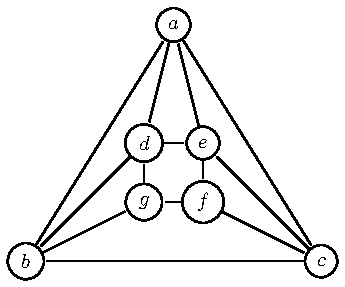
\includegraphics[scale=.8]{8_1.pdf}
\end{center}

\begin{enumerate}
	\item Determine $\chi(G)$.

	\begin{center}
		\tikz
		\graph [no placement] {
			a [x=0cm,y=0cm, red] -- b [x=-2cm,y=-4cm, blue] -- c [x=2cm,y=-4cm, green] -- e [x=0.5cm,y=-2cm, blue] -- d [x=-0.5cm,y=-2cm, green] -- g [x=-0.5cm,y=-3cm, red] -- f [x=0.5cm,y=-3cm]; 
			g--b--d--a--e--f--c--a;
		};
	\end{center}
	I am not sure if the printer used in printing these sheets does color, but I colored the graph with 4 colors. To show there can't be less than 4, assume there is a coloring of 3. $\{a,b,d\}$ must all be different colors, and $\{b,d,g\}$ must all be different colors, so $a$ and $g$ must be the same color, we'll call color 1. Similar reasoning makes $d$ and $c$ the color 2, and $b$ and $e$ color 3. $f$ is adjacent to $g$, $e$, and $c$, so $f$ must be a color different from all of those. \Therefore the chromatic number of this graph is 4. \micdrop

	\item Is $G$ color-critical? If so, prove that $\chi(G-e) < \chi(G)$ for every edge $e \in E(G)$. If not, find a color-critical subgraph of $G$.
\end{enumerate}
	
\medskip
	
\item Prove that for any graph $G$, there exists an ordering of $V(G)$ for which the greedy algorithm uses exactly $\chi(G)$ colors.
	
\medskip
	
\item Let $G$ be a graph. Prove or disprove the following statements.
\begin{enumerate}
	\item There exists a $\chi(G)$-coloring of $G$ in which one color class contains $\alpha(G)$ vertices.\m
	I will disprove this conjecture by making a counter example.
	\begin{center}
		\tikz \graph[grow right=1cm, branch down=1cm, nodes={circle,draw}] {
			{[nodes = blue] a,b,c} -!- {[nodes = {xshift = 1cm, red}] d,e,f};
			a -- {e,f};
			d -- {a,b,c}
		};
	\end{center}
	Each class has 3 vertices, and the largest independent set is $\{b,c,e,f\}$.
	\item $\chi(G) \leq 1 + \overline{d}(G)$ where $\overline{d}(G)$ is the {\em average degree} in $G$. 
	
	\item $\chi(G) \leq n-\alpha(G)+1$.
	\begin{proof}
		Since the other two statements were disprovable, using the Theorem of human predictability and probabilistic method, we know this statement is provable.\\
		Let $G$ be a $n$-vertex graph. Give every vertex it's own color. We have a coloring of $n$ colors. Let us take the set of the largest independent set. Since the set has no edges between them, we can recolor those vertices as just 1 color. And now we have a valid coloring of $n-\alpha(G)+1$.
	\end{proof}
\end{enumerate}
	
\medskip
\item Let $G$ be an $n$-vertex graph. Prove that $\chi(G)\cdot\chi(\overline{G}) \geq n$, and use this to prove $\chi(G) + \chi(\overline{G}) \geq 2\sqrt{n}$. For each $n$ where $\sqrt{n}$ is an integer, construct a graph that achieves both equalities.
	
\begin{proof}
	
\end{proof}
	
\medskip
	
{\em Hint: using a $\chi(G)$-coloring of $G$ and a $\chi(\overline{G})$-coloring of $\overline{G}$, construct a proper coloring of $K_n$. Also you may find it useful to use the AM-GM inequality which states that if $x$ and $y$ are non-negative real numbers, then $\sqrt{xy} \leq \frac{x+y}{2}$.}
	
\medskip
\item Let $G$ be an $n$-vertex graph. Prove that $\chi(G) + \chi(\overline{G}) \leq n+1$ and conclude that $\chi(G) \cdot \chi(\overline{G}) \leq [(n+1)/2]^2$. For each odd $n$, give an example of a graph $G$ that achieves both equalities.
\footnote{From questions 3 and 4, we obtain that for every graph $G$ on $n$ vertices, either $G$ or its complement has chromatic number at least $\sqrt{n}$, and either $G$ or its completement has chromatic number at most $(n+1)/2$.}
 
\medskip

{\em Hint: use induction to prove $\chi(G) + \chi(\overline{G}) \leq n+1$.}


\end{enumerate}
\end{document}
